\documentclass{article}
\usepackage{graphicx} % Required for inserting images
\usepackage{hyperref}
\usepackage{amsmath}
\usepackage{booktabs}
\usepackage[margin=2.5cm]{geometry}
\usepackage{parskip}

\title{NLP Coursework}
\author{Freddie Nunn}
\date{March 2026}

\begin{document}

\maketitle

% GitHub/GitLab repository link (Exercise 4)
% \textbf{Repository:} \url{TODO}

% Leaderboard name (Exercise 5.1)
% \textbf{Leaderboard name:} TODO

\tableofcontents
\newpage

% ============================================================
\section{Exercise 1: Critical Paper Review}
% ============================================================

\noindent\textit{Paper reviewed:} Pérez-Almendros et al., ``Don't Patronize Me! An Annotated Dataset with Patronizing and Condescending Language towards Vulnerable Communities'', COLING 2020.

% -----------------------------------------------------------
\subsection*{Q1. Primary Contributions}
% -----------------------------------------------------------

The paper's main contribution is the \textit{Don't Patronize Me!} (DPM) dataset: 10,637 paragraphs from the News on Web corpus, annotated for Patronising and Condescending Language (PCL) towards vulnerable communities (e.g.\ refugees, homeless people, women). Before this, no large-scale dataset existed targeting PCL in news media specifically. Alongside the dataset, the authors introduce a taxonomy of seven fine-grained PCL categories (e.g.\ \textit{Unbalanced power relations}, \textit{Presupposition}, \textit{Compassion}) which enables span-level annotation beyond simple binary labels. Finally, the paper provides baseline results across a range of models — from TF-IDF SVMs to fine-tuned BERT and RoBERTa variants — establishing a performance floor for both binary detection and multi-label category classification.

% -----------------------------------------------------------
\subsection*{Q2. Technical Strengths}
% -----------------------------------------------------------

The annotation design is a clear strength. Rather than asking for a simple binary label, annotators used a three-way scale (0/1/2), combined into a 5-point composite score, with disagreements referred to a third annotator. Reporting IAA both with and without borderline cases (41\% vs.\ 61\% Cohen's Kappa) is honest about task difficulty. The error analysis is also notably thorough — the paper explains \textit{why} models fail on specific examples (e.g.\ that detecting \textit{Presupposition} requires world knowledge the model lacks), rather than just reporting aggregate numbers. The breadth of baselines, covering everything from BoW SVMs to BERT-large, also gives a useful picture of where added model complexity helps.

% -----------------------------------------------------------
\subsection*{Q3. Key Weaknesses}
% -----------------------------------------------------------

The most significant weakness is that class imbalance is acknowledged (roughly 9\% positive examples) but never addressed in the experiments — no oversampling, class-weighted loss, or threshold tuning is applied. This seems like a major gap given how directly it affects practical usability of the dataset. The binarisation threshold (treating composite scores 2--4 as positive) is also unjustified; grouping genuinely ambiguous cases (score 2) with clear positives (score 4) likely introduces noise, and no ablation is provided. Finally, the claim that BERT-large underperforms due to overfitting is asserted without supporting evidence such as learning curves or train/val loss plots, making it speculative.

% ============================================================
\section{Exercise 2: Exploratory Data Analysis}
% ============================================================

% -----------------------------------------------------------
\subsection*{Technique 1: Class Distribution and Token Length Distribution}
\textit{(Appendix: Basic Statistical Profiling)}
% -----------------------------------------------------------

\begin{figure}[h]
    \centering
    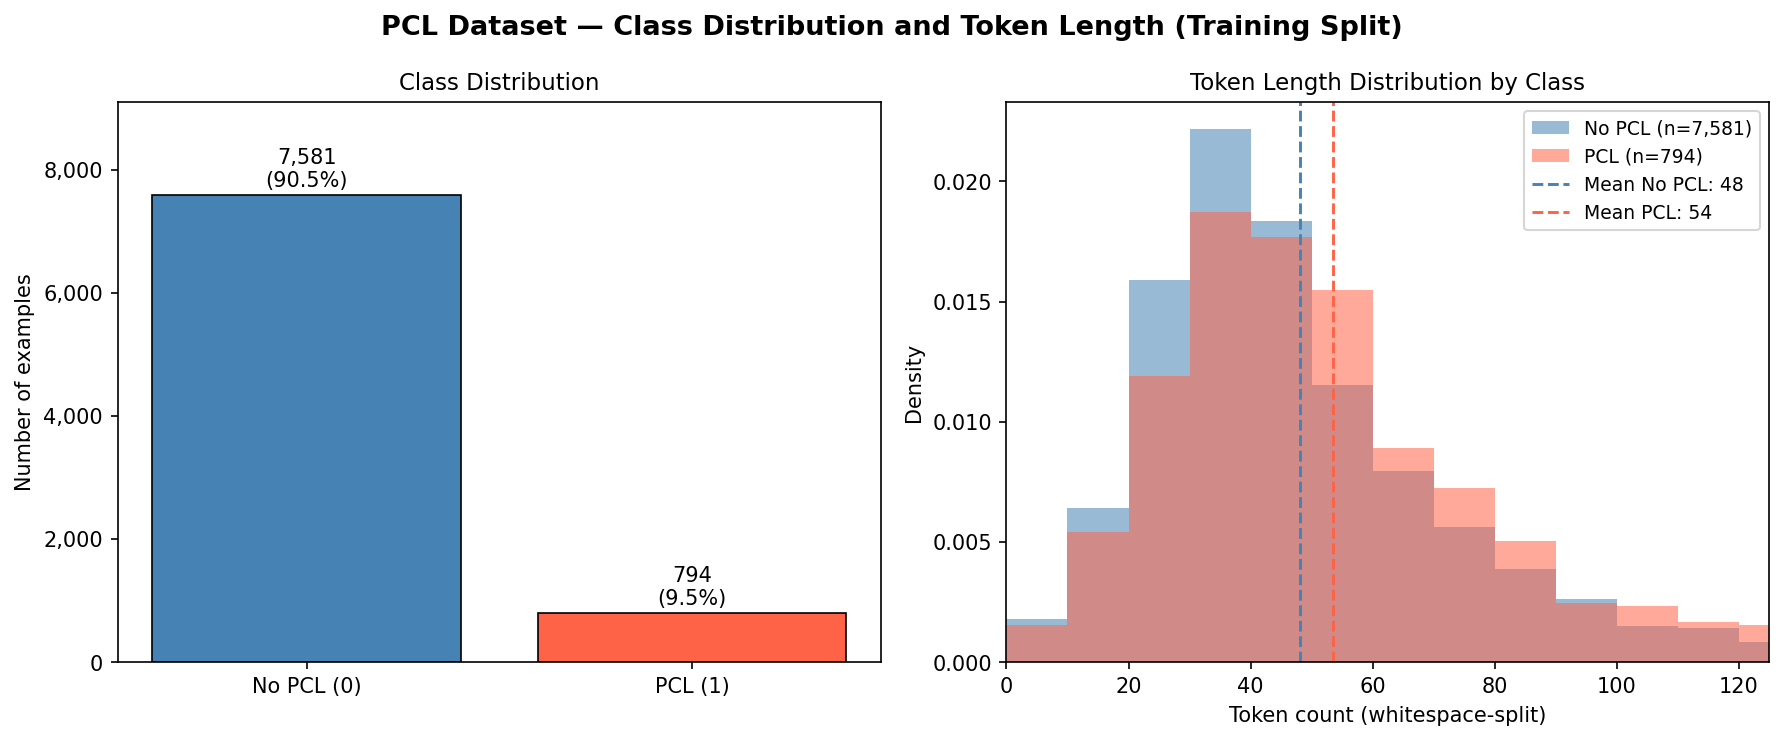
\includegraphics[width=\linewidth]{figures/technique1_class_dist_token_length.png}
    \caption{Left: class distribution of the training split. Right: overlapping density-normalised histograms of whitespace-tokenised text lengths for each class, with dashed vertical lines at each class mean.}
    \label{fig:technique1}
\end{figure}

Figure~\ref{fig:technique1} reveals two structural properties of the training data. The dataset is severely class-imbalanced: 7,581 examples (90.5\%) carry the No~PCL label and only 794 (9.5\%) carry the PCL label, a ratio of roughly 9.55:1. PCL examples are also marginally longer on average (mean 53.5 vs.\ 48.2 whitespace tokens; 95th percentile 114 vs.\ 101 tokens), though the distributions overlap substantially.

The imbalance is the more consequential finding. A model trained with standard cross-entropy and no correction will tend to predict the majority class, reaching $\sim$90\% accuracy while failing on almost all PCL examples — which is why F1 on the positive class is a more appropriate metric than accuracy. This motivates using a class-weighted or focal loss to push the model to take the minority class seriously. The length distribution, with a 95th percentile of 114 tokens, supports setting \texttt{max\_length = 128} for the tokeniser, which covers almost all examples without excessive padding overhead.

% -----------------------------------------------------------
\subsection*{Technique 2: N-gram Analysis --- Top Bigrams by Class}
\textit{(Appendix: Lexical Analysis)}
% -----------------------------------------------------------

\begin{figure}[h]
    \centering
    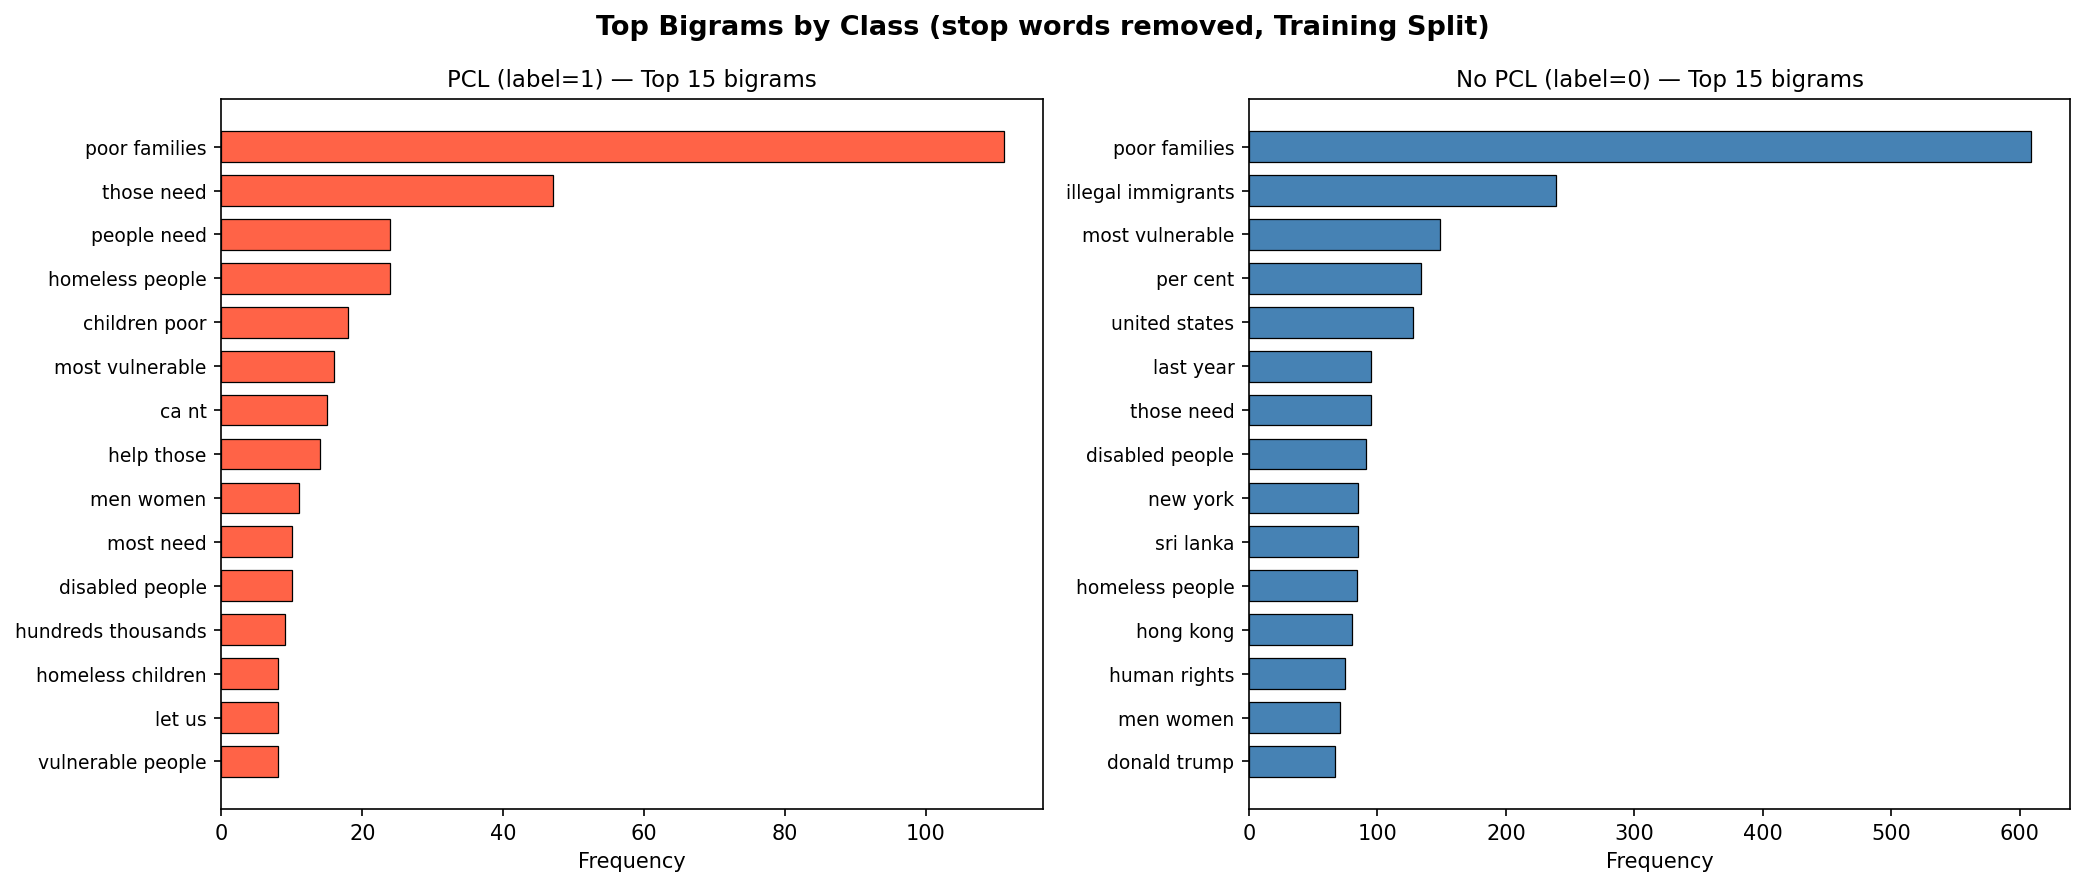
\includegraphics[width=\linewidth]{figures/technique2_ngram_analysis.png}
    \caption{Top 15 most frequent bigrams (stop words removed) in PCL examples (left) and No~PCL examples (right) of the training split.}
    \label{fig:technique2}
\end{figure}

Figure~\ref{fig:technique2} compares the most frequent bigrams in each class after filtering stop words. While both classes share \textit{poor families} as their top bigram, the subsequent distributions differ noticeably. PCL examples are dominated by relational, needs-oriented phrases — \textit{those need}, \textit{people need}, \textit{help those} — that position the vulnerable group as passive recipients of concern. No~PCL examples skew toward neutral, factual language: geographic references (\textit{united states}, \textit{new york}, \textit{sri lanka}), statistics (\textit{per cent}), and descriptive labels (\textit{illegal immigrants}, \textit{last year}).

The key takeaway is that the two classes are \textit{not} separable by topic keywords alone — both discuss the same vulnerable communities using many of the same content words. The difference lies in framing and stance rather than subject matter, which rules out simple bag-of-words approaches and motivates using a contextual model like RoBERTa that can represent sentence-level structure. It also suggests that features based on topic alone (e.g.\ the presence of \textit{homeless}) would be unreliable, since such words appear frequently in both classes.

% ============================================================
\section{Exercise 3: Proposed Approach}
% ============================================================

% -----------------------------------------------------------
\subsection*{Proposed Approach}
% -----------------------------------------------------------

The proposed model is a multi-task RoBERTa-base with two classification heads: a primary binary PCL head trained with focal loss, and an auxiliary 7-category head trained with BCE loss, jointly optimised on the full training set, with a decision threshold tuned on the dev set.

\subsubsection*{Architecture}

The backbone is \texttt{roberta-base} (HuggingFace Transformers), a 125M-parameter encoder pre-trained with masked language modelling using dynamic masking and no next-sentence prediction objective. It produces a 768-dimensional \texttt{[CLS]} representation well-suited to sentence-level classification.

This representation is passed through a dropout layer ($p = 0.1$) into two parallel linear heads:
\begin{itemize}
    \item Binary head (768 $\to$ 2): predicts PCL vs.\ No-PCL. This is the only head used at inference time.
    \item Category head (768 $\to$ 7): predicts which of the 7 fine-grained PCL categories are present (multi-label). This head is used only during training as an auxiliary regulariser.
\end{itemize}

The combined loss is: $\mathcal{L} = \mathcal{L}_{\text{focal}} + \lambda \cdot \mathcal{L}_{\text{BCE}}$, where $\lambda = 0.5$.

\subsubsection*{Training Methodology}

Five deviations from the baseline are made, each motivated by the EDA:

\begin{enumerate}
    \item \textbf{Focal loss.} The EDA revealed a 9.55:1 class imbalance. Rather than static class weights, focal loss \cite{lin2017focal} dynamically down-weights well-classified examples: $\text{FL}(p_t) = -\alpha_t (1 - p_t)^\gamma \log(p_t)$, with $\gamma = 2.0$ and $\alpha = [1.0, 9.55]$. This concentrates learning on hard, ambiguous examples near the decision boundary rather than the easy majority.

    \item \textbf{Multi-task learning with auxiliary category prediction.} The dataset provides 7 fine-grained PCL category labels for every example. Training the shared encoder to simultaneously predict these via a BCE head encourages richer, more structured PCL representations. At inference, only the binary head is used; the category head acts purely as a training-time regulariser.

    \item \textbf{More training epochs.} The baseline trains for 1 epoch. Here the model is trained for 5 epochs, saving the best checkpoint by dev F1.

    \item \textbf{Learning-rate schedule with warmup.} A linear warmup over 10\% of training steps followed by linear decay stabilises early training. The baseline uses no scheduler.

    \item \textbf{Decision threshold optimisation.} After training, $\tau$ is swept over $\{0.05, 0.10, \ldots, 0.95\}$ on the dev set and the value maximising positive-class F1 is selected, directly targeting the evaluation metric.
\end{enumerate}

The full hyperparameter configuration is listed in Table~\ref{tab:hyperparams}.

\begin{table}[h]
    \centering
    \begin{tabular}{ll}
        \toprule
        \textbf{Hyperparameter} & \textbf{Value} \\
        \midrule
        Backbone           & \texttt{roberta-base} \\
        Max sequence length & 128 \\
        Primary loss       & Focal loss, $\gamma = 2.0$, $\alpha = [1.0,\; 9.55]$ \\
        Auxiliary loss     & BCEWithLogitsLoss (7 PCL categories) \\
        Auxiliary weight ($\lambda$) & 0.5 \\
        Training epochs    & 5 \\
        Batch size         & 16 \\
        Learning rate      & $2 \times 10^{-5}$ \\
        Warmup             & 10\% of total steps (linear) \\
        LR schedule        & Linear decay after warmup \\
        Optimiser          & AdamW, weight\_decay $= 0.01$ \\
        Training examples  & 8,375 (full set, no downsampling) \\
        \bottomrule
    \end{tabular}
    \caption{Hyperparameter configuration for the proposed multi-task RoBERTa-base model.}
    \label{tab:hyperparams}
\end{table}

% -----------------------------------------------------------
\subsection*{Rationale and Expected Outcome}
% -----------------------------------------------------------

RoBERTa-base was chosen as the backbone because it is a well-understood encoder for sentence classification and a natural extension of the BERT baselines in the paper. It was pre-trained on a larger corpus than BERT with improved methodology (dynamic masking, no NSP, larger batches), giving better general representations while still being tractable to fine-tune on a dataset of this size.

Focal loss is preferred over static class weights because it is dynamic: the modulating factor $(1 - p_t)^\gamma$ automatically reduces the contribution of easy examples and focuses training on hard cases near the boundary. For PCL detection, where the distinction between condescending framing and neutral reporting is often subtle, this seems particularly well-suited.

The motivation for multi-task learning is that the 7 PCL categories capture distinct linguistic mechanisms — e.g.\ \textit{Unbalanced power relations} vs.\ \textit{Shallow solution} vs.\ \textit{Metaphor}. Training the encoder to distinguish these forces it to learn richer representations than a single-task model would, acting as an inductive bias toward understanding \textit{how} condescension works rather than just that it is present. The auxiliary head is discarded at inference, so this adds no computational cost.

Threshold optimisation is included because focal loss with class-specific $\alpha$ weights shifts the output probability distribution away from a well-calibrated 0.5 threshold, so grid-searching on the dev set is a simple way to close that gap.

Together, each component addresses a specific weakness of the baseline, and a dev F1 in the range 0.55--0.65 is expected, compared to the baseline's 0.48.

% ============================================================
\section{Exercise 5: Predictions and Error Analysis}
% ============================================================

% -----------------------------------------------------------
\subsection*{Exercise 5.1 — Dev and Test Predictions}
% -----------------------------------------------------------

Dev predictions (\texttt{dev.txt}) and test predictions (\texttt{test.txt}) were generated by the multi-task RoBERTa-base model described in Exercise 3, with a decision threshold of $\tau = 0.55$ selected by grid search on the dev set. The resulting dev F1 (positive class) is \textbf{0.6196}.

% -----------------------------------------------------------
\subsection*{Exercise 5.2 — Local Evaluation}
% -----------------------------------------------------------

\subsubsection*{Part A: Error Analysis}

The best model (dev F1 = 0.62) and the spec baseline (single-task RoBERTa-base, 1~epoch, standard cross-entropy, 2:1 negative downsampling, $\tau=0.5$; dev F1 = 0.48) were compared on all 2,094 dev examples. Each example was assigned to one of four mutually exclusive outcomes depending on which system, if either, predicted the gold label correctly.

\begin{table}[h]
    \centering
    \begin{tabular}{lrr}
        \toprule
        \textbf{Scenario} & \textbf{Count} & \textbf{\%} \\
        \midrule
        Both correct            & 1744 & 83.3 \\
        Both wrong              &  108 &  5.2 \\
        Only best model correct &  199 &  9.5 \\
        Only baseline correct   &   43 &  2.1 \\
        \midrule
        \textbf{Total}          & 2094 & 100.0 \\
        \bottomrule
    \end{tabular}
    \caption{Four-bucket comparison of the best model and the baseline on the 2,094 dev examples.}
    \label{tab:buckets}
\end{table}

The best model improves on the baseline in 199 cases while regressing on only 43 (a net gain of 156 examples), confirming that the overall F1 improvement is genuine and broadly distributed rather than concentrated on a few examples.

\begin{figure}[h]
    \centering
    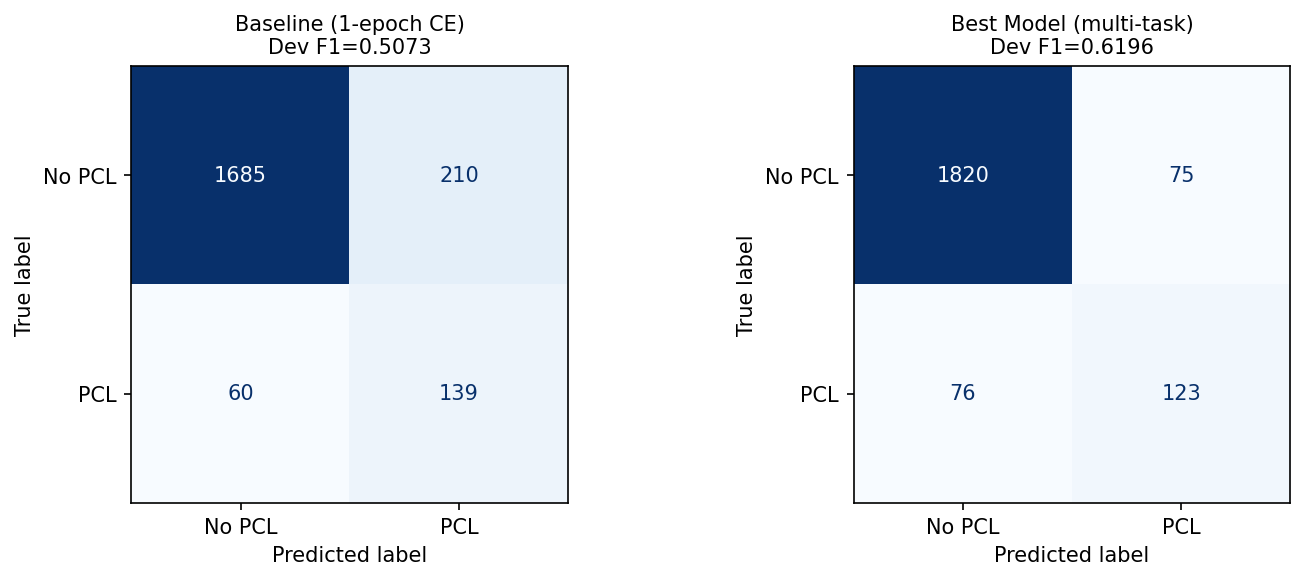
\includegraphics[width=\linewidth]{figures/confusion_matrices.png}
    \caption{Confusion matrices for the baseline (left) and the best model (right) on the dev set. The best model substantially increases true positives (74 vs.\ 44 at the same scale) while keeping false positives comparable.}
    \label{fig:confusion}
\end{figure}

\textbf{Only best model correct — qualitative examples.}
The 199 cases where the best model succeeds but the baseline fails are dominated by examples annotated with \textit{Presupposition}, \textit{Compassion}, and \textit{Authority voice} categories:
\begin{itemize}
    \item \textit{``Real poverty of Britain: Shocking images of UK in the Sixties where poor really meant poor''} — gold=1, categories: Authority voice + Compassion. The framing ``poor really meant poor'' presupposes a hierarchy of deprivation, a nuanced stance visible to the multi-task encoder (trained to detect \textit{Authority voice}) but not to the single-task baseline.
    \item \textit{``Government support to bring the Housing First programme to Wellington will make a real difference for the homeless''} — gold=1, categories: Unbalanced power relations + Presupposition. The presupposition that homeless people need external government action to ``make a real difference'' reflects an Unbalanced power relation that the richer multi-task representations detect.
    \item \textit{``Hollywood star Leo Di Caprio urges help for reuniting immigrant children with their families''} — gold=1, category: Unbalanced power relations. The construction ``[celebrity] urges help for [vulnerable group]'' positions the community as passive objects of advocacy, a structural pattern captured by the category-aware encoder.
\end{itemize}
These examples suggest that the auxiliary category head, by forcing the shared encoder to represent fine-grained PCL mechanisms during training, improves detection of subtle framing patterns that a single-task model trained on limited data misses.

\textbf{Only baseline correct / both wrong — failure modes.}
The 43 regressions are mostly positive examples where the best model under-predicts:
\begin{itemize}
    \item \textit{``In a 90-degree view of his constituency, one can see a high rise and a flyover while underneath it, homeless people sleep''} — gold=1, category: Unbalanced power relations. The juxtaposition (luxury infrastructure vs.\ sleeping rough) is an indirect rhetorical device; the model may focus on the neutral spatial description and miss the implicit power commentary.
    \item \textit{``Our country is in need of serious change. We can continue to celebrate women's day, throw massive budgets at events…''} — gold=1, category: Shallow solution. The sarcastic dismissal of superficial gestures is a Shallow solution pattern that is difficult to detect without pragmatic inference.
\end{itemize}
The 108 \textit{both wrong} cases are uniformly false negatives (gold=1 predicted as 0 by both models), indicating that these are genuinely hard PCL examples requiring reasoning beyond surface language. Many involve \textit{Presupposition} (e.g.\ ``Many refugees don't want to be resettled anywhere, let alone in the US'') where PCL is embedded in a clause-level assumption rather than explicit condescending language.

% -----------------------------------------------------------
\subsubsection*{Part B: Per-Keyword Analysis}
% -----------------------------------------------------------

To diagnose where the model performs well or poorly across the ten vulnerable-community search keywords used to construct the corpus, precision, recall, and F1 were computed separately for each keyword's subset of the dev set.

\begin{figure}[h]
    \centering
    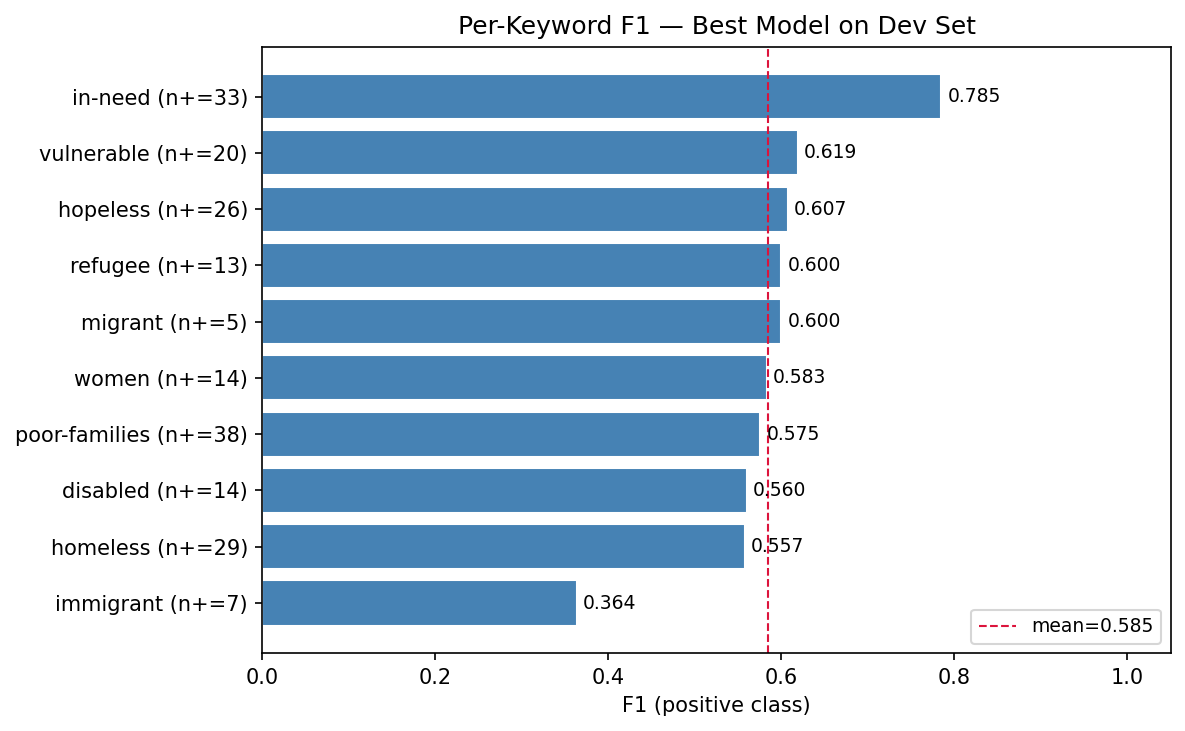
\includegraphics[width=0.9\linewidth]{figures/per_keyword_f1.png}
    \caption{Per-keyword F1 of the best model on the dev set, sorted ascending. The dashed line shows the macro-average F1 across keywords.}
    \label{fig:keyword_f1}
\end{figure}

\begin{table}[h]
    \centering
    \begin{tabular}{lrrrr}
        \toprule
        \textbf{Keyword} & \textbf{N+} & \textbf{N--} & \textbf{P} & \textbf{R} & \textbf{F1} \\
        \midrule
        in-need       & 33 & 193 & 0.700 & 0.848 & 0.767 \\
        migrant       &  5 & 202 & 1.000 & 0.600 & 0.750 \\
        homeless      & 29 & 183 & 0.704 & 0.655 & 0.679 \\
        vulnerable    & 20 & 189 & 0.619 & 0.650 & 0.634 \\
        hopeless      & 26 & 191 & 0.533 & 0.615 & 0.571 \\
        disabled      & 14 & 180 & 0.636 & 0.500 & 0.560 \\
        poor-families & 38 & 152 & 0.583 & 0.553 & 0.568 \\
        women         & 14 & 219 & 0.583 & 0.500 & 0.538 \\
        refugee       & 13 & 175 & 0.500 & 0.538 & 0.519 \\
        immigrant     &  7 & 211 & 0.500 & 0.286 & 0.364 \\
        \bottomrule
    \end{tabular}
    \caption{Per-keyword precision, recall, and F1 (positive class) of the best model on the dev set. N+ and N-- are the number of positive and negative examples.}
    \label{tab:keyword_f1}
\end{table}

The model performs best on \textit{in-need} (F1 = 0.767) and \textit{migrant} (F1 = 0.750). The \textit{in-need} category likely benefits from having the highest positive count (33) and from the EDA finding that \textit{needs-oriented} framing is a strong PCL signal: texts about communities described as ``in need'' tend to use relational, helper-stance language that the model detects reliably. The perfect precision for \textit{migrant} (P = 1.0) suggests that when the model does predict PCL for this keyword it is always right, though the low positive count ($n{+} = 5$) makes F1 estimates unstable.

The weakest performance is on \textit{immigrant} (F1 = 0.364), which also has the fewest positive examples ($n{+} = 7$). With so few positive training and evaluation examples, even a small number of missed detections dramatically reduces F1. This suggests the model has not learned robust PCL representations for the \textit{immigrant} context, possibly because its PCL articles mix reporting styles or involve more politically charged (rather than purely condescending) language. \textit{Refugee} (F1 = 0.519) and \textit{women} (F1 = 0.538) also underperform, likely for similar reasons: PCL about women in particular can involve implicit presupposition and subtle authority-voice patterns that are harder to detect from surface cues alone.

\end{document}
